\lstdefinestyle{mystyle}{
    backgroundcolor=\color{CadetBlue!15!white},   
    commentstyle=\color{Red3},
    numberstyle=\tiny\color{gray},
    stringstyle=\color{Blue3},
    basicstyle=\small\ttfamily,
    breakatwhitespace=false,         
    breaklines=true,                 
    numbers=left,                    
    numbersep=5pt,                  
    showspaces=false,                
    showstringspaces=false,
    showtabs=false,                  
    tabsize=2,
    language=C
}%
\lstset{language=C,style={mystyle}}%


\chapter{Técnicas útiles}
En este capítulo veremos algunas técnicas utilizadas en las siguientes secciones. Estas son, por ejemplo, usos particulares de patrones de diseño.


\section{Desacople de módulos}

A lo largo de los ejemplos del documento, veremos repetidas veces el uso de la noción de \textit{orden} o \textit{comando}. Cada vez que sea nombrado haremos referencia a la aplicación de un patrón de diseño de Gamma \cite{Gamma:1995:DPE:186897}, el patrón \textit{Command}. 

La función principal que cumple este patrón es la de desacoplar el objeto que invoca una orden, la orden en si y aquel que sabe como llevarla a cabo. Es decir, reemplaza las \textit{callbacks} entre módulos. Como objetivo fundamental, buscamos no tener que modificar la implementación del módulo invocador en caso de un cambio en el que se encarga de realizar las tareas. Ademas, se le quita la responsabilidad de saber exactamente que acciones realizar para llevar a cabo un procedimiento particular. Por ejemplo, un módulo necesita que otro se inicie, pero este ultimo para hacerlo requiere que se invoque una serie de sus funciones de manera ordenada. Si lo hacemos de la forma clásica, el primer módulo debe ajustar su implementación al segundo. En cambio, con una orden movemos la responsabilidad a un nuevo módulo.

\begin{figure}
\caption{Estructura patrón \textit{Command}}
\begin{center}
\begin{tikzpicture}\sf
\umlsimpleclass[]{Invocador}
\umlclass[right=2cm of Invocador,type=abstract]{Orden}
{}
{
\umlvirt{ejecutar()}
}
\umlclass[below=2cm of Invocador]{Receptor}
{}
{
acción
}

\umlclass[below=1.45cm of Orden]{OrdenConcreta}
{}
{
ejecutar()
}

\umluniassoc{OrdenConcreta}{Receptor}
\umlinherit{OrdenConcreta}{Orden}
\umluniaggreg{Invocador}{Orden}

\end{tikzpicture}
\end{center}
\end{figure}

\begin{itemize}
    \item \textbf{Invocador}: le pide a la Orden que ejecute la acción.
    \item \textbf{Orden}: declara la interfaz para ejecutar una acción.
    \item \textbf{OrdenConcreta}: implementa la función ejecución la cual se encarga de llamar la o las funciones del \textbf{Receptor} con el objetivo de llevar a cabo la acción.
    \item \textbf{Receptor}: cualquier clase, es sobre la cual se realiza la acción.
\end{itemize}
Al encapsular cada solicitud de una operación dentro de un objeto, el patrón permite que los módulos que incovan acciones no necesiten conocer los detalles de implementación de los módulos que las ejecutan. Esto reduce significativamente las dependencias y hace que el sistema sea más fácil de mantener, ya que cada módulo se concentra en su propia responsabilidad, sin acoplarse a los detalles de otros módulos. 
El patrón \textit{Command} es una herramienta efectiva para lograr el desacoplamiento entre módulos en sistemas complejos, especialmente útil cuando se busca modularidad y flexibilidad en la organización de comandos y acciones. Al encapsular cada solicitud de una operación dentro de un objeto de comando, el patrón \textit{Command} permite que los módulos que emiten instrucciones no necesiten conocer los detalles de implementación de los módulos que las ejecutan. Esto reduce significativamente las dependencias y hace que el sistema sea más fácil de mantener, ya que cada módulo se concentra en su propia responsabilidad, sin acoplarse a los detalles de otros módulos. Además, la extensión de funcionalidades se simplifica considerablemente. Dado que cada acción está representada por un módulo independiente, se pueden agregar nuevos comandos al sistema sin modificar los módulos existentes. Esta estructura es particularmente útil cuando se necesita modificar o añadir funcionalidades de manera frecuente. Al mismo tiempo, los comandos encapsulados pueden almacenarse, reutilizarse y combinarse en secuencias, lo que facilita la implementación de operaciones complejas que se repiten o que requieren ser acumuladas para un procesamiento posterior. Por otro lado, como el comando es un módulo puede ser extendido para implementar múltiples funcionalidades, como deshacer operaciones o registrar cambios. 

\begin{figure}[h]
\caption{Ejemplo de aplicación básica del patrón \textit{Command}}
\begin{center}
\begin{tikzpicture}\sf
\umlsimpleclass[]{Controller}
\umlclass[right=2cm of Controller]{MotorGirarIzq}
{}
{
ejecutar()
}
\umlclass[below=1cm of Controller]{Motor}
{}
{
right() \\
left() \\
disable() \\
enable() \\
pulse()
}

\umlnote[below=1cm of MotorGirarIzq]{MotorGirarIzq}{
ejecutar() \{ \\
\ \ \ \ motor.enable() \\
\ \ \ \ motor.left() \\
\ \ \ \ motor.pulse() \\
\}
}


\end{tikzpicture}
\end{center}
\end{figure}

El módulo \textbf{Controller} aplicará la acción de girar el motor a la izquierda un paso sin saber como llevarla a cabo específicamente. Y en caso de que el motor cambie, solo debemos modificar la orden, e incluso podemos dejar la existente y crear una nueva con la nueva implementación.

En caso de no aplicar el patrón tendríamos todo el código que se encarga de girar el motor hacia la izquierda en \textbf{Controller}, como en el código \ref{notCommand}.

\begin{lstlisting}[label={notCommand}, caption=Ejemplo de implementación sin usar el patrón \textit{Command}.]
control() {
    .
    .
    .
    motor.enable()
    motor.left()
    motor.pulse()
    .
    .
    .  
}
\end{lstlisting}

En caso de que el modo de operación del motor cambie deberemos modificar el código del método \verb|control|.

Otro uso interesante del patrón, es cuando se define una cierta estructura conceptual en el sistema. Esta puede responder a la naturaleza de la aplicación del mismo. Por ejemplo, en un sistema de control, se puede definir que los módulos que realizan el control del mismo invoquen a los sensores para obtener información. Generando así, una cierta jerarquía en la cual los sensores no deben invocar métodos de módulos superiores. En caso de ser necesaria la comunicación de manera inversa se puede hacer uso del patrón \textit{command} para reemplazar el uso de \textit{callbacks}.


